\documentclass[border=4pt]{standalone}
\usepackage{amsmath,amssymb}
\usepackage{tikz}
\begin{document}
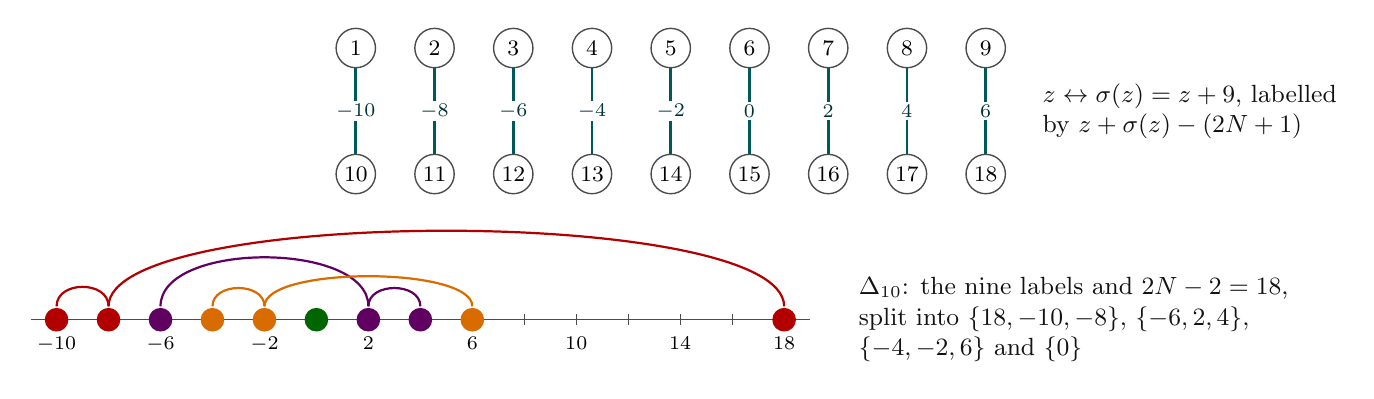
\begin{tikzpicture}[
  x=1cm, y=1cm,
  note/.style={font=\small,gray!15!black,align=left,anchor=west},
  dot/.style={circle,draw=black!70,fill=white,line width=0.5pt,inner sep=0pt,minimum size=5mm,font=\footnotesize},
  val/.style={font=\scriptsize,fill=white,inner sep=1pt,text=teal!40!black}]
  % N = 10, K = 18: sigma(z) = z + 9 for 1 <= z <= 9
  \foreach \z in {1,...,9} {
    \pgfmathtruncatemacro{\w}{\z+9}
    \pgfmathtruncatemacro{\d}{2*\z-12}
    \draw[teal!70!black,line width=1pt] (\z,-0.25) -- (\z,-1.35);
    \node[val] at (\z,-0.8) {$\d$};
    \node[dot] at (\z,0) {$\z$};
    \node[dot] at (\z,-1.6) {$\w$};
  }
  \node[note] at (9.6,-0.8) {$z\leftrightarrow\sigma(z)=z+9$, labelled\\ by $z+\sigma(z)-(2N+1)$};
  % Delta_N on a line
  \begin{scope}[yshift=-3.45cm, x=0.33cm, xshift=0.5cm]
    \draw[gray!60!black,line width=0.5pt] (-11,0) -- (19,0);
    \foreach \x in {-10,-8,...,18} { \draw[gray!60!black] (\x,0.07) -- (\x,-0.07); }
    \foreach \x in {-10,-6,-2,2,6,10,14,18} { \node[font=\scriptsize,anchor=north] at (\x,-0.1) {$\x$}; }
    \foreach \x/\col in {18/red!70!black, -10/red!70!black, -8/red!70!black,
                         -6/violet!75!black, 2/violet!75!black, 4/violet!75!black,
                         -4/orange!85!black, -2/orange!85!black, 6/orange!85!black, 0/green!40!black} {
      \fill[\col] (\x,0) circle (1.5mm);
    }
    \draw[red!70!black,line width=0.8pt] (-10,0.17) .. controls (-10,0.5) and (-8,0.5) .. (-8,0.17);
    \draw[red!70!black,line width=0.8pt] (-8,0.17) .. controls (-8,1.45) and (18,1.45) .. (18,0.17);
    \draw[violet!75!black,line width=0.8pt] (-6,0.17) .. controls (-6,1.0) and (2,1.0) .. (2,0.17);
    \draw[violet!75!black,line width=0.8pt] (2,0.17) .. controls (2,0.48) and (4,0.48) .. (4,0.17);
    \draw[orange!85!black,line width=0.8pt] (-4,0.17) .. controls (-4,0.48) and (-2,0.48) .. (-2,0.17);
    \draw[orange!85!black,line width=0.8pt] (-2,0.17) .. controls (-2,0.68) and (6,0.68) .. (6,0.17);
    \node[note] at (20.5,0) {$\Delta_{10}$: the nine labels and $2N-2=18$,\\ split into $\{18,-10,-8\}$, $\{-6,2,4\}$,\\ $\{-4,-2,6\}$ and $\{0\}$};
  \end{scope}
\end{tikzpicture}
\end{document}
